%
% File acl2018.tex
%
%% Based on the style files for ACL-2017, with some changes, which were, in turn,
%% Based on the style files for ACL-2015, with some improvements
%%  taken from the NAACL-2016 style
%% Based on the style files for ACL-2014, which were, in turn,
%% based on ACL-2013, ACL-2012, ACL-2011, ACL-2010, ACL-IJCNLP-2009,
%% EACL-2009, IJCNLP-2008...
%% Based on the style files for EACL 2006 by 
%%e.agirre@ehu.es or Sergi.Balari@uab.es
%% and that of ACL 08 by Joakim Nivre and Noah Smith

\documentclass[11pt,a4paper]{article}
\usepackage[hyperref]{acl2018}
\usepackage{times}
\usepackage{latexsym}
\usepackage{graphicx}
\usepackage[center]{caption}
\usepackage{float}
\usepackage{hyperref}
\usepackage{caption}
\captionsetup{font=footnotesize}
\usepackage{indentfirst}

\usepackage{url}


\aclfinalcopy 
%\def\aclpaperid{***} %  Enter the acl Paper ID here

%\setlength\titlebox{5cm}
% You can expand the titlebox if you need extra space
% to show all the authors. Please do not make the titlebox
% smaller than 5cm (the original size); we will check this
% in the camera-ready version and ask you to change it back.

\newcommand\BibTeX{B{\sc ib}\TeX}

\title{Classical Art Memes}

\author
  {Clara Helmig\\
  {clara.helmig\\@stud.uni-regensburg.de} \\\And
  {Janina Schatz\\
  janina.schatz\\@stud.uni-regensburg.de}  \\\And
  {Daniel-Alexander Vikete \\
 { daniel-alexander.vikete\\@stud.uni-regensburg.de}
  }}

\date{28.04.2023}

\begin{document}
\maketitle
\begin{abstract}
Memes have become an integral part of everyday life on the internet in relation to social media. They can be found on all popular platforms and on platforms like Reddit and 9 Gag they make up a large part of the posts.
This paper deals with the analysis of the subgenre Classical Art Memes.
The first step is to scrape the memes from a subreddit and collect them in a corpus. The text is then identified using OCR and subjected to common analysis methods to extract POS tagging, NER, word frequency and sentiment. The images are also analysed for differences in brightness (sentiment comparison).
\end{abstract}

\section{Introduction}
Memes are of great importance in today's world, as they have become increasingly relevant, especially in recent years during the Corona Pandemic \cite{Barnes2021}. According to \citeauthor{Bauckhage2021} (\citeyear{Bauckhage2021}), “Internet memes are inside jokes or hip knowledge from the underground, that are shared by many people”.
Memes are shared by people through forums,
blogs, and especially social media websites like
Reddit, Facebook, Twitter and Pinterest. Internet
memes are based on imitations, parodies and
current events in the world \cite{Bauckhage2021}.
They spread very quickly on the Internet, some of
them
\begin{figure}[H]
    \centering
    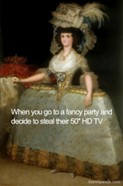
\includegraphics[scale=1]{acl18-latex/Bild1.jpg}
    \caption{Most upvoted post on the subreddit '\hyperlink{https://www.reddit.com/r/trippinthroughtime/}{trippingthroughtime}'}
    \label{fig:my_label}
\end{figure}
trending on social media for only a few days \cite{Barnes2021}. One category of memes is the so-called "Classical Art Memes," which will be examined in this paper. The term "classical art" is usually understood to refer to the much broader category of visual art produced in the style of classicism \cite{Lanci2022}. Thus, Classical Art Memes refer to a variety of humorous image macros based on paintings and other visual artworks that predate modern history. Image macros are an alternative term for static image and text, which refers to reusable images that are typically embedded in a background that is repeated often and are accompanied by a text \cite{Laineste2017}. An example for this can be seen in figure 1.
Computational research on memes is currently a rather unexplored area in the field of social media analysis. Our project builds on the few studies and investigations on memes that have already been completed, which is another reason why we want to devote ourselves to the phenomenon of Classical Art Memes. This project can serve as further inspiration for projects in both social media analysis and art research. 
The goal of this study is threefold. First, a meme corpus was created based on a subreddit. Next, an image data analysis was to be performed to identify the original artworks. However, this objective could not be achieved. Instead, a general analysis of the images was conducted, which proved successful. We will then evaluate the textual component of the memes using fundamental text analysis techniques. Overall, the purpose of this study is to shed more light on the significance and relevance of Classical Art Memes in online culture as well as the manner in which these images are utilized and changed in the modern era. In the following point related researches and studies are shown. Afterwards the methods of this work are explained. Based on this, the results of our research are presented. The results are then deliberated in the discussion. As a second to last point the limitations are pointed out. Finally, the most important points
are summarized in the conclusion.

\section{Related Work}
Research on the specific mass phenomenon of Classical Art Memes is currently limited. However, existing work provides a starting point for further investigation. In the Related Work section, an overview of previous studies and research dealing with the analysis of Classical Art Memes is presented. Firstly, general studies are presented that deal with the linguistic and visual analysis of memes and the role they play in online communication. Then, specific studies on Classical Art Memes are discussed. These studies deal with different aspects such as recipient behaviour, communication within the community, or the mystery of "funny" memes. These studies provide insights into different perspectives on Classical Art Memes. They also show that In addition, it becomes clear that the lower-level way of looking at Classical Art Memes is a new one and offers a new perspective on this niche of memes and communication on the Internet.
That memes are not a subgenre in the Internet and social media world is shown by \citeauthor{wiggins2015} (\citeyear{wiggins2015}) in their study on 'memescape'. They analyzed the interaction of the individual elements (image, text, context) and the role of memes in digital culture. They have also shown their influence in politics, identity and adulation. They have found out that the particular structure of images plays an essential role in the emergence and spread of viral phenomena. Users know this and consciously use memes to spread certain topics. They were able to identify three different meme catgoirs: spreadable, emergent, meme. Memes usually contain mixed and repetitive messages. \citeauthor{wiggins2015} show that memes played no small role in social media and Internet culture, but memes can be seen as a cultural genre in digital culture.  In general, memes can function in different cultures with different political and social contexts. Memes have come to be an important dominant role in memes. The fact that memes can indeed carry an opinion and also influence other people is confirmed by \citeauthor{Osterroth2019} (\citeyear{Osterroth2019}) in his study on memes in public discourse using the example of the reply threads in Donald Trump's account. In his work, he focused on memes created by users in response to Donald Trump's tweets. He examined both visual and linguistic elements. \citeauthor{Osterroth2019} believes that memes convey a message that is not always obvious at first glance, as the recipient has to combine image and writing to fully grasp the content. On the one hand, he was able to show in his study that meems are used as a means for olitical discourse and can thus represent a variety of different opinions. On the other hand, he showed that a meme functions as a multimodal speech act and thus contributes to strengthening or weakening political positions.
\\
\\ \citeauthor{Raivio2016} investigated the relationship between meme and user in \citeyear{Raivio2016}. According to him Classical Art Memes do not only influence the real-life experience but can also be seen as part of a person's own experience in the virtual world. He also conducted an investigation into the themes, topics and moods of Classical Art Memes. Here, he found that the memes often feature portraits, religious content, or manipulated images. \citeauthor{Raivio2016} attributes this to the fact that the artworks were created in a time when only nobles could afford art, and also to the fact that Western Europe was initially mostly religious. The subjects of these images were varied and included war, animals, sex, relationship, mythology, among others. The manipulated images show that here,
too, artistic past meets modernity.
\\Addressing the question of what constitutes humor in memes, \citeauthor{Piata2019} (\citeyear{Piata2019}) understands Classical Art Memes as a special category of memes in her 2020 research. Because only in this kind of memes artistic past is combined with contemporary text of modern situations. This new connection leads to a new interpretation of the artwork. And this has a great impact on online humor. \citeauthor{Piata2019} describes that humor is triggered by the interaction of image and text. The image in the meme is the way people could feel but only with the corresponding text in the meme it makes sense and describes modern life. This unexpected meeting of the two elements leads to the triggering of the humor response. For this finding, she examined 130 memes. Here it turned out that all clear facial expressions (surprise, fear, sadness etc.) which are universally recognizable, were represented. Through the simple recognition of the images and a modern reference through the text, emotions are thus triggered in the viewer. \citeauthor{Piata2019} believes that this simple approach brings viewers closer to classic works of art.
\\ \citeauthor{alluri2021} (\citeyear{alluri2021}) examined about 700
memes to see if they contained sarcasm and humor. Similarly, they sought to determine the motivation behind the posting and the sentiment triggered. \citeauthor{alluri2021} divided each meme into two categories at a time (funny/not funny; sad/not sad, etc.). Subsequent research was largely based on working with Transformer models that had both, image and text embeddings. Thus, they use 'VisionTransformer' to filter out the most influential elements in the image. 'BERT' was then used for text analysis because the model is both a maskedlanguage model and can make next-sentence predictions. The subtitles of each meme were evaluated using RESNET-weighted transformer models (IMGTXT, RoBERTa, IMGSEN). Therefore, all three models gave different results depending on the category (Accuracy: 62.77\%, F1 score 59.045\%). Thus, they were able to detect humor and sarcasm based on machine evaluation of memes.
\\The fact that consumers of memes are emotionally addressed by the Meme itself was also found by \citeauthor{Vlachou2022} (\citeyear{Vlachou2022}). They examined the relationship between posts from museum visitors and their emotions, as well as the
polarity of memes and the artworks displayed in them. In the dataset of 250,000 Classical Art Memes (Instagram), they additionally determined the most viral (a meme was considered viral if the artwork shown occurred more than ten times in the dataset). Using Google Image Search, they looked up the artist, work name, and the museum where the artwork is currently present. By analyzing museum posts, comments, and likes, they were able to make the following connection: Museum visitors were emotional when they saw a work of art in the museum that they had seen before on various memes. Thus, there was a high recognition value. It can be concluded that the digital age has a significant impact on the aesthetic experience in the museum.
So, we see that there is a lot of research on the effect of memes on their viewers. Likewise, there are some studies that address the popularity of Classical Art Memes in general. But to our knowledge there are no studies including computer vision techniques and Classical Art Memes. 

 \section{Methods}
 The methods we used to collect, examine, and compare the Classical Art Memes is described in the chapter that follows.
 \subsection{Data Acquisition}
To start with it was attempted to download the relevant information from the "trippinthroughtime" subreddit. Instead the data was downloaded directly from the Pushshift dump page. In doing so, the data was too large to be downloaded all at once. For this reason, one file after the other was downloaded, processed, and then deleted.\footnote{https://www.reddit.com/r/pushshift/comments/ajmcc0\\/comment/ef012vk/}
The following metadata was stored in the CSV file: score, author, total\_awards\_received, created\_utc, num\_comments, selftext, title, url, domain, permalink, id, subreddit\_subscribers,num\_crossposts, relative\_path. The number of posts between 2015 and 2022 was 40,365.
Then the data was cleaned. All posts not ending with png or jpg and all duplicates were deleted and the results were written to a new CSV file. The cleaned CSV file was then implemented to download the images using the included URL. If the download was successful, the images were saved in the images folder. The images that failed to download because they were not present (HTTP status code 404) were stored separately in a log file and then deleted from the dataframe. The result was a data set with 28,109 entries.
\par
The next goal was to recognize the text contained in the images and convert it into machine-readable text. For this purpose, optical character recognition (OCR) was applied to the images. The captured text was to be stored in a new column "ocr\_text" in the dataframe and written to a new CSV file. 
To make the accuracy of the results as high as possible, different approaches for OCR were tested. First, pytesseract\footnote{https://pypi.org/project/pytesseract/} was tried in conjunction with the Python package PIL (Python Imaging Library)\footnote{https://pillow.readthedocs.io/en/stable/}. Pytesseract provides an interface to the Tesseract OCR engine and is an OCR tool that can work with various image formats and recognize text in multiple languages.\cite{Imtiaz2020}
The image was first opened with the PIL library, converted to grayscale, and the contrast was increased to ensure better readability of the text during extraction. However, the results did not have the desired level of accuracy. For example, text that was not black on white was not recognized. 
It was also tested instead of PIL to preprocess the images with cv2. Here the image is converted to grayscale, smoothed, i.e. noise and other artifacts are removed, and binarized, i.e. the image pixels are converted to black and white. Despite the additional processing steps of cv2, the results were very similar to those obtained with PIL. 
Therefore, the Google Cloud Vision API\footnote{https://cloud.google.com/vision/docs/ocr?hl=de}
was subsequently applied for text recognition, which is also suitable for large amounts of images and promises a better recognition rate. With the Google Vision API, the images can be sent to the API without preprocessing. The recognized text is returned in a JSON format. From these JSON files, the text is stored in a CSV file.  Since this method had the highest accuracy, we proceeded implementing this technique.
\par
After OCR, some images had to be excluded from the dataset as they were images without content. Also, some memes existed in the dataset (N = 1,086) that did not contain text. These were manually examined and it was determined that the relevant text was in the Reddit title of the post. For this reason, the blank OCR texts were replaced with the post title. Some Reddit users posted the same image multiple times. These duplicates were deleted. The resulting, cleaned dataset numbered 23375 posts which were then used for further analysis. The column names and their description can be found in \autoref{tab:columns}. 


\begin{table*}[h]
  \centering
  \begin{tabular}{|l|l|}
    \hline
    \textbf{Attribute} & \textbf{Description}\\
    \hline
    \rowcolor[gray]{0.9} score & Score of the submission\\
    \hline
    author & ID of the user who wrote the submission  \\
    \hline
    \rowcolor[gray]{0.9} total\_awards\_received & Total number of awards received by the submission\\
    \hline
    created\_utc & Time the submission was created, represented in Unix Time\\
    \hline
    \rowcolor[gray]{0.9} num\_comments & Number of comments on the submission \\
    \hline
    selftext & The text of the submission, if it is a selfpost \\
    \hline
    \rowcolor[gray]{0.9} title & The title of the submission \\
    \hline
    url & The URL associated with the submission \\ 
    \hline
    \rowcolor[gray]{0.9} domain & The domain associated with the submission \\
    \hline
    permalink & The permanent URL of the submission \\ 
    \hline
    \rowcolor[gray]{0.9} id & The ID of the submission \\ 
    \hline
    subreddit\_subscribers & The number of subscribers to the subreddit where the submission was made \\ \hline
    \rowcolor[gray]{0.9} num\_crossposts & The number of times the submission has been cross-posted to other subreddits \\ 
    \hline
    relative\_path & The relative path of the image file associated with the submission \\ 
    \hline
    \rowcolor[gray]{0.9} file\_name & The name of the image file associated with the submission \\ 
    \hline
    ocr\_text & The text detected in the image file associated with the submission \\ 
    \hline
  \end{tabular}
  \caption{column names and description}
  \label{tab:columns}
\end{table*}


 \subsection{Data Analysis}
 \textbf{General Corpus Analysis}:
 Different approaches were used for the analysis of the corpus. For natural language processing (NLP) with Python, respectively for preprocessing, the language processing library spaCy \cite{Luber2020}
 was used. The "en\_core\_web\_sm"\footnote{https://spacy.io/models/en#en\_core\_web\_sm} model was used. It is one of the smaller and faster models for the English language and is suitable for many NLP applications. The OCR texts were subjected to tokenization and the type-token ratio (TTR) was obtained. The TTR is understood as the ratio of the number of distinct, unique words (tokens) to all words in the text. The TTR is thus a measure of how diverse and varied a text is.
 \cite{Wimmer2005}
In addition, the measure of textual lexical diversity (MTLD) was obtained, which is a useful method that has a higher correlation with human assessments of text complexity than other measures. The "lexicalrichness" library was utilized to calculate several measures of lexical diversity in the text. The text was first processed with spaCy, tokenized and added to the "Lexical Richness Object". The MTLD is calculated with a threshold of 0.72, as recommended by McCarthy and Jarvis.\cite{McCarthy2010}
Furthermore, some statistics, such as the number of posts, awards, comments, score and subscribers were determined for each year in order to get an overview and to be able to make statements about possible correlations.
 \par
 \textbf{Sentiment Analysis}: Sentiment analysis was performed utilizing the OCR text. To run sentiment analysis with Python there are several options. In this project NLTK-Vader (Natural Language Toolkit- Valence Aware Dictonary and Sentiment Reasoner) was used. NLTK-Vader is a part of the NLTK library and is able to classify texts into different sentiment categories (positive, neutral, negative) \cite{Ma2020}. Words or single sentences can be rated and the sentiment score can be summed up. In this way, an overall score is obtained for the entire text. NLTK-Vader is based on the original Vader; it is an updated version that was developed especially for social media texts. This way, expressions like 'lol' or 'smh' as well as emojies are also taken into account. For this reason, NLTK-Vader is well suited for the OCR text of Classical-Art-Memes. The module uses about 7500 words and scores. Each element can have a negative (-4) or positive intensity (+4). A value of 0 corresponds to a neutral sentiment score. Similarly, reinforcements are included in the calculation of sentiment. Although NLTK-Vader is based on a trained lexicon with associated sentiment categories, some phrases and expressions that are common in the meme language may still not be in the lexicon. 
 \par
 \textbf{POS and NER}: In order to perform a meaningful Part-of-Speech-Tagging (POS) and Named-Entity-Recognition (NER) procedure, the OCR text must first be cleaned up. Thus, all words were converted into lowercase words and the punctuation was removed. Likewise, the stop words were removed using the nltk.stopword list. The text was tokenized and the website watermarks were deleted. In addition to tokenization, the words were also subjected to lemmatization.
 \textbf{POS-Tagging} is a method to identify word types in a text. This allows for the identification of various parts of speech such as nouns, verbs, adverbs, pronouns, and conjunctions within the text \cite{Luber2022}. Not covered here are the different forms of each word in person, tense, numerus and case, etc. \textbf{NER} is a similar process to POS. Here, too, different words are analyzed, identified and divided into categories. In contrast to POS tagging, no word types are distinguished, but entities are determined. The NER module of NLTK uses a machine learning process to identify entities like persons, places, organizations, data or products. For this project, NER is important to identify persons like Jesus, Zeus or Mom and organizations like tech companies or pharmaceutical companies and schools. Both methods were performed after submission of NLTK documentation \cite{nltk2021}. The code was applied to each year's OCR text and returns a new column with all the words and their POS-tag/ NER. Then all POS-tags/ NER are calculated with NLTK-FreqDisk and the ten most frequent tags/NER were determined. Then the POS/NER categories and their respective frequencies were extracted from the tags. The ten most frequent words were plotted in a bar chart.
 \par \textbf{Word Frequency}: The last analysis step for text processing deals with word frequency. Using simple Python functions, the column containing the OCR text was analyzed. Applying a counter class from the Collections module, the frequency of each word was counted. Subsequently, the output was visualized either as a bar chart and as a graphical word cloud.
 \par
 \textbf{Computer Vision}: A major goal of this project was to perform image analysis. The objective was to determine which images, created by which artists, from which historical periods, and with which motifs, were most commonly employed in the creation of memes. Several methods were tried in Python. A direct analysis of images was conducted using reference images.  For this, memes were loaded into one folder and an original artwork was loaded into another folder. The goal was to match the correct meme with the original artwork. Three different analysis methods were available: SSIM, ORB and HOG. SSIM (Structural Similyrity Index) mainly compares brightness and contrast of the images \cite{Datta2020}. Thus, the code converted all images into RBG colors and compares the gray levels. The ORB (Oriented Fast and Rotated Brief) method uses two factors simultaneously for analysis \cite{Tyagi2019}. FAST (Features from Accelerated Segment Test) finds points with high intensity and BRIEF (Binary Robust Independent Elementary Features) converts them into binary patterns. This way, especially features like edges and corners can be compared with each other. HOG (Histogram of Oriented Gradients) looks for the important gradients of the image based on brightness and color \cite{Mallick2016}. This basically creates black images with white pixels, which can be compared more easily. Unfortunately, none of the three approaches could match a meme with the original work or the original work with the correct meme.
Therefore, a new approach was tested. An attempt was made using the reverse Google Image search. The code entered the meme into Google Search, called the first hit, and used Beautiful-Soup to parse the site by artist and title. Another attempt accessed the Wiki Art page via the Wiki Art API, matched the image to the database, and returned the best possible match. Unfortunately, these attempts were not successful.
\par We believe that the lack of success in our search was due to limitations within the dataset, prompting us to manually search for relevant artists and artworks. However, this approach proved to be ineffective as even a manual search for a meme from the dataset only yielded similar memes on other websites. To accurately match the meme images with their original sources, some form of processing is required. However, this is beyond the scope of our current project and will need to be addressed in future research.
\newline \par One way to analyze the images without going into their origin is to examine the images themselves. Therefore, the color choice of the images was investigated. Colors in artworks transport feelings and influence the viewer's emotions \cite{Schels2020}.A barcode diagram was used for a pictorial representation of the colors \cite{CainnD}. The barcodes were based on the average color of the memes. The color code is a visual representation of the dominant colors of the images, with each image representing a single color bar in the barcode. Next, the average color of the image was calculated from the pixel values obtained along both axes. Then a color bar is created with the average color \cite{Chen2021}.
 \section{Results}
 \textbf{General Corpus Analysis}:
 The number of tokens in the OCR texts was 606,076 (\autoref{tab:Token}). Derived from this, the type-token ratio provided a value of 0.0887. Only 8.87\% of the tokens are thus unique tokens, which may indicate that the texts contains relatively little variation in vocabulary. Related to the context of Classical Art Memes, this can be attributed to the fact that this is a concrete type of meme that often uses certain recurring keywords and terms. Contrarily, the MTLD value is at a relatively high level of around 128.8, which means that the text has a high lexicality. This, in turn, is an indication that the text is multifaceted. The TTR value and the MTLD value in combination can be explained as the text having a sufficient number of diverse words despite the use of repeated keywords and terms, and thus the MTLD value is at this high level. Classical Art Memes are often humorous or ironic, and a varied text helps to reinforce the punchline and mood of the meme, making the text enjoyable and easy to read.
 
\begin{table}[h]
  \centering
  \begin{tabular}{|c|c|}
   \hline
     & Value \\
    \hline
    \rowcolor[gray]{0.9} Token & 606076 \\
    \hline
    TTR & 0.0887 \\
    \hline
    \rowcolor[gray]{0.9} MTLD & 128.7674 \\
    \hline
  \end{tabular}
  \caption{Token, TTR \& MTLD}
  \label{tab:Token}
\end{table}

 
 The number of posts reached its peak in 2019 and 2020, with significantly high user activity during these years (\autoref{fig:year-wise}). This can be attributed to the SARS-CoV-2 pandemic and the given measures, which led to the fact that people spent significantly more time at home versus previous years. The increasing number of comments and subscribers can be explained analogously.(\autoref{fig:comments},\ref{fig:subscribers} ) 
 \begin{figure}[H]
    \centering
    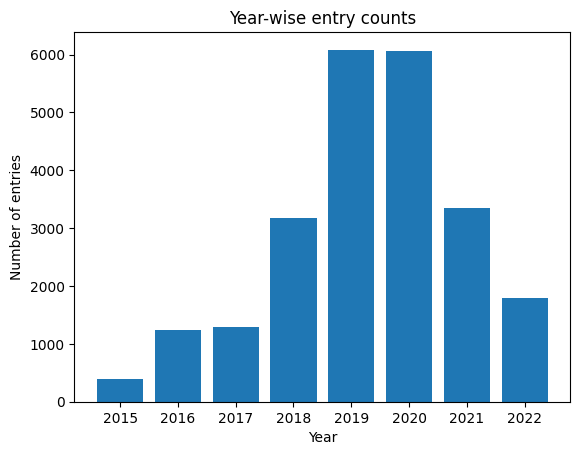
\includegraphics[scale=0.5]{acl18-latex/image_count_year.png}
    \caption{Year-wise entry counts}
    \label{fig:year-wise}
\end{figure}
\begin{figure}[H]
    \centering
    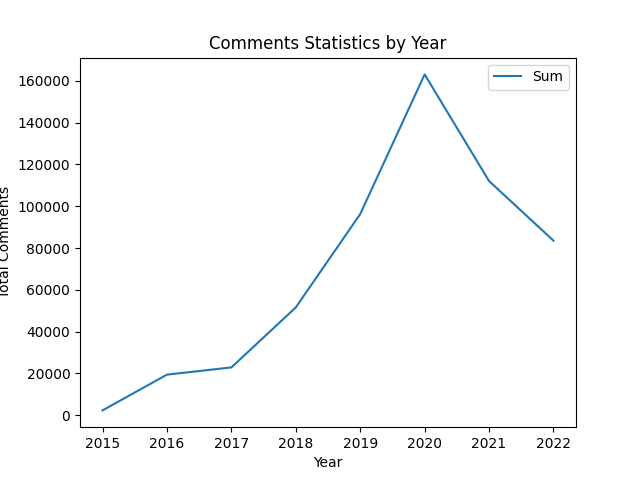
\includegraphics[scale=0.5]{acl18-latex/comments_stats.png}
    \caption{Comments statistics by year}
    \label{fig:comments}
\end{figure}
\begin{figure}[H]
    \centering
    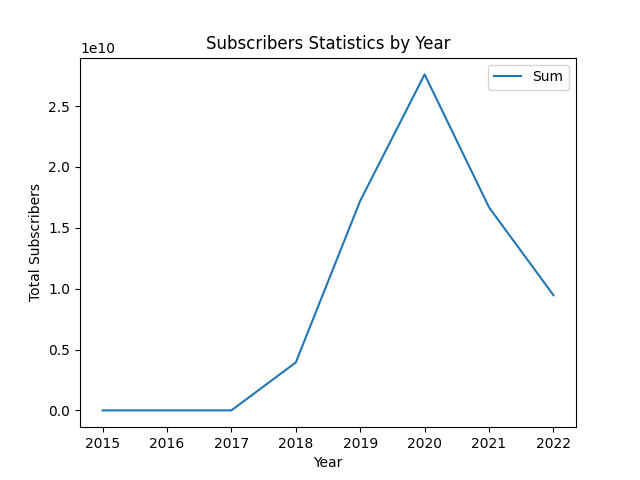
\includegraphics[scale=0.5]{acl18-latex/subscribers_stats.png}
    \caption{subscribers statistics by year}
    \label{fig:subscribers}
\end{figure}
\vspace{-4cm}
\begin{figure}[H]
    \centering
    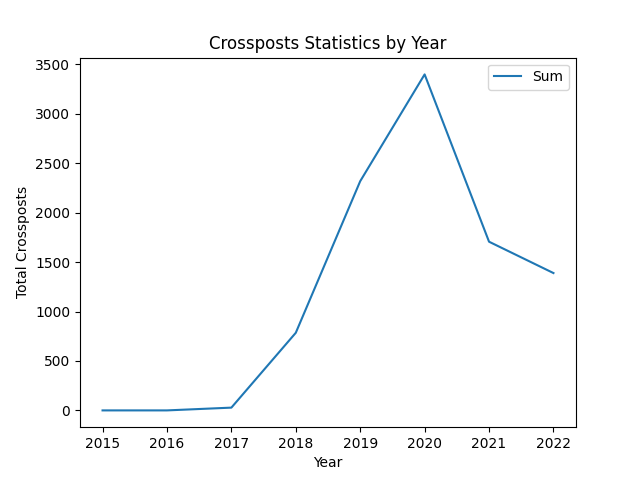
\includegraphics[scale=0.5]{acl18-latex/crossposts_stats.png}
    \caption{Crossposts statistics by year}
    \label{fig:crossposts}
\end{figure}
Additionally, the increasing number of crossposts (\autoref{fig:crossposts}) goes hand in hand with the previously mentioned assumptions of increased online engagement and the need for humor. Furthermore, one could conclude that during the pandemic, the sense of community and togetherness played an increasing role in a time of limited social contact and isolation and, consequently, community building took place here in a different way. 
\begin{figure}[H]
    \centering
    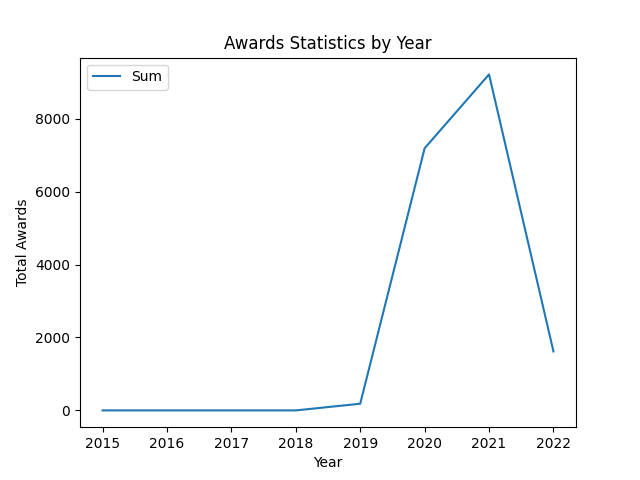
\includegraphics[scale=0.5]{acl18-latex/awards_stats.png}
    \caption{Awards statistics by year}
    \label{fig:awards}
\end{figure}
By 2021, the number of awards (\autoref{fig:awards}) had reached its highest point, which could be explained by the increasing popularity that had been growing since 2019.
\begin{figure}[H]
    \centering
    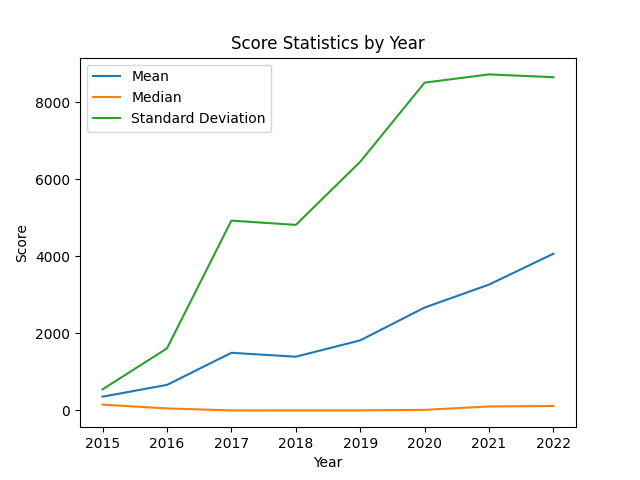
\includegraphics[scale=0.5]{acl18-latex/score_stats.png}
    \caption{Score statistics by year}
    \label{fig:score}
\end{figure}
Reddit uses a scoring system to indicate the overall rating of a post by its users. The score of a submission reflects its positive or negative rating, with higher scores indicating more positive ratings. The almost constant median of the scores over time indicates that their distribution is relatively stable and thus the users generally assign similar ratings to the posts. The median score has increased, likely due to the rise in posts with higher scores over time, which has contributed to the increase in the overall average (\autoref{fig:score}). As explained in the beginning, this can also be attributed to higher user activity. The sharp increase in the standard deviation shows that the score values have become more widely spread over time, which suggests an increased number of extreme ratings and controversial posts.

 \par
 \textbf{Sentiment Analysis}: As previously described, the sentiment score was calculated using NLTK-Vader. If we look at the distribution of the sentiment score over the years, the following picture emerges (Figure \ref{fig:Figure Average Sentiment}):
 \begin{figure}[H]
    \centering
    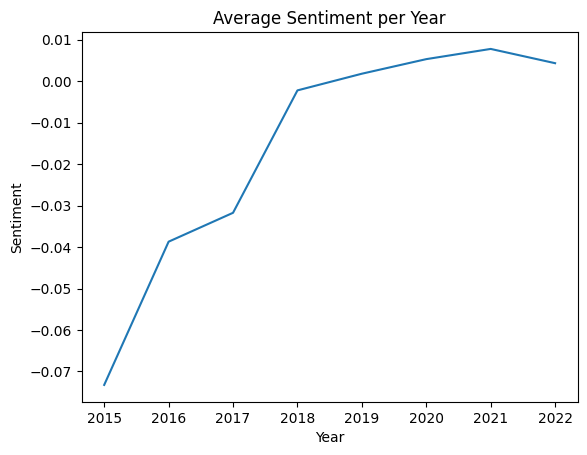
\includegraphics[scale=0.5]{acl18-latex/Sentiment Result 1.png}
    \caption{Average Sentiment per Year}
    \label{fig:Figure Average Sentiment}
\end{figure}
\vspace{-0.4cm}
The graph rises over the years with a peak in 2021. However, upon closer inspection of the data, the total sentiment score for each year only increases by a small margin, from -0.07 to +0.01. This is due to the fact that the sentiment score can range from -1 to +1, and the observed change of 0.08 is such a small difference in this range. Instead, we took a look at the percentage distribution (Figure \ref{fig: Average Sentiment Percentagel})  of positive/neutral/negative memes in order to make a more differentiated statement about the sentiment score.
\begin{figure}[H]
    \centering
    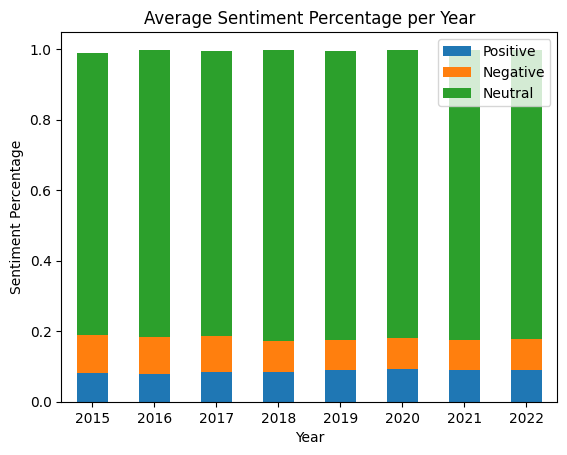
\includegraphics[scale=0.5]{acl18-latex/Sentiment Result 2.png}
    \caption{Average Sentiment Percentage per Year}
    \label{fig: Average Sentiment Percentagel}
\end{figure}
Noticeable is the high proportion of sentences with a neutral recognition score. This may be due to some expressions from the subreddit not being included in NLTK-Vader's lexicon. No better fitting module was found, which could also be applied for social media texts. The sentences that were assigned a clear sentiment direction were distributed to both positive and negative sentiments. Thus, despite the non-ideal lexicon, the sentences were neutral. In order to confirm this fact unambiguously, a model or module is needed with a suitable lexicon, or a fine-tuned model for the 'language of classical art memes'.
\par\textbf{POS-Tagging}:
 Following are the POS-Charts for 2015 ( \autoref{fig: POS 2015}) for 2022 ( \autoref{fig:POS 2022}) for comparison:
 \begin{figure}[H]
    \centering
    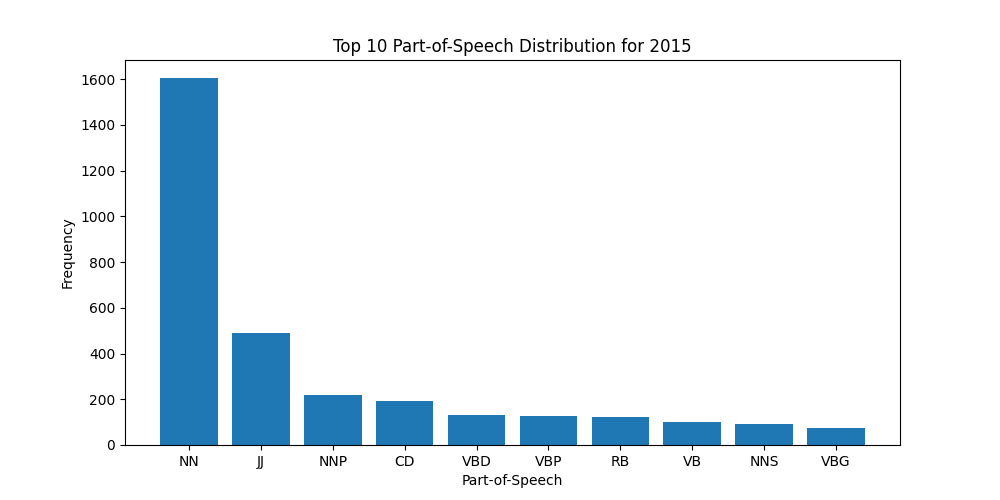
\includegraphics[scale=0.35]{acl18-latex/POS 2015.png}
    \caption{TOP 10 POS-Distribution in 2015}
    \label{fig: POS 2015}
\end{figure}
 
 \begin{figure}[H]
    \centering
    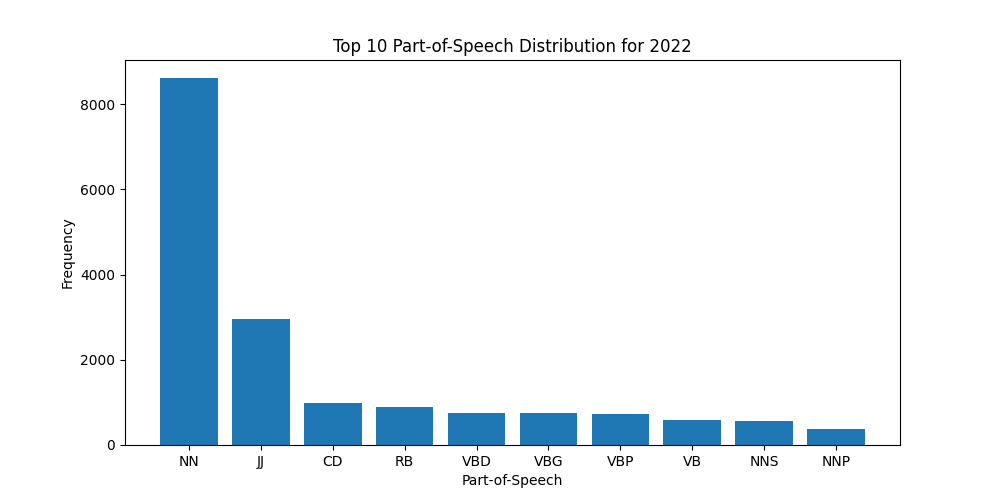
\includegraphics[scale=0.35]{acl18-latex/POS 2022.png}
    \caption{TOP 10 POS-Distribution in 2022}
    \label{fig:POS 2022}
\end{figure}
If we look at all the bar charts of the POS distributions over the years, we see that in absolute terms there were more words  in 2022. However, their relative proportion in the individual categories remained the same. Only their order had changed.
\textbf{NER}: If we have a look at the distribution of the NER, we can see that the top 4 word types are the same in all years. There are almost the same types of words in the top 10 in 2015, 2019 and 2022:  
\\\newline
\begin{center}
    \begin{tabular}[h]{l|c|r}
        2015 & 2019 & 2022  \\
        \hline
         \rowcolor[gray]{0.9} Cardinal & Cardinal & Cardinal\\
         Person & Person & Person\\
         \rowcolor[gray]{0.9} Date & Date & Date \\
         ORG & ORG & ORG \\
         \rowcolor[gray]{0.9} GPE & GPE & GPE\\
         Time & Time & Time\\
         \rowcolor[gray]{0.9} Ordinal &  NORP & NORP\\
         NORP & Ordinal & Ordinal \\
         \rowcolor[gray]{0.9} FAC &  Quantity &  Product\\
         Quantity & Product & Quantity
        \label{tab:TOP NER}    
    \end{tabular}\newline
\end{center}    

There are only small shifts in placement. However, when looking at the absolute numbers of NERs found, this is probably not very meaningful.
Particular attention should be paid to the top 4 or 5. These are mainly numbers, personal names and organisations. It should be noted that our NER programme has found a cardinal number and not a date from the year 1023. For the system to recognise a date, at least two out of three entries must be given (e.g. 04.09 or May 1934). This may explain the high number of cardinal numbers. A look at the persons found shows that Jesus, old gods, you and mum play the main roles in classical art memes.
\newline \par
\textbf{Word Frequency}: \autoref{fig:Word Cloud 2015} and \ref{fig:Word Cloud 2019} show the most frequent words as a wordcloud in 2015 and 2016, respectively. As you can see there are many swear words like 'fuck' or 'bitch' in the images.
\begin{figure}[H]
    \centering
    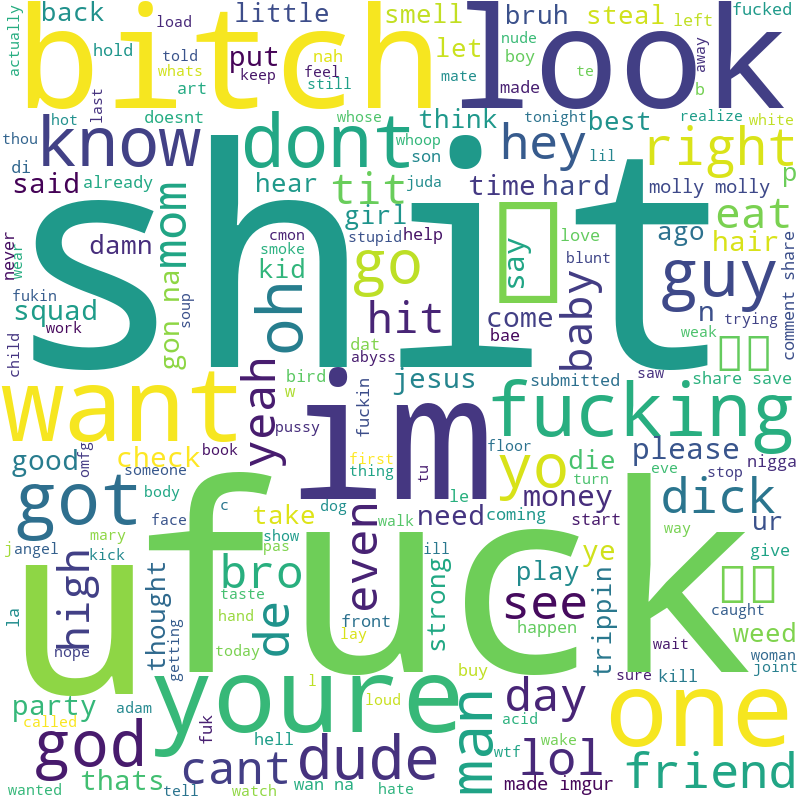
\includegraphics[scale=0.2]{acl18-latex/word_cloud_2015_ocr_text.png}
    \caption{Most frequent Words 2015}
    \label{fig:Word Cloud 2015}
\end{figure}

\begin{figure}[H]
    \centering
    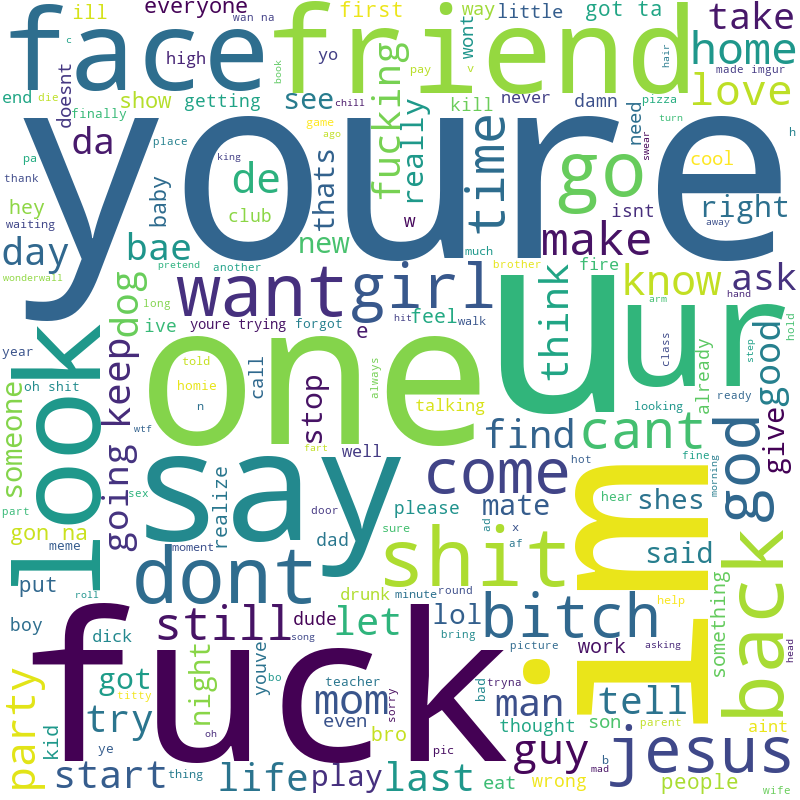
\includegraphics[scale=0.2]{acl18-latex/word_cloud_2016_ocr_text.png}
    \caption{Most frequent Words 2016}
    \label{fig:Word Cloud 2019}
\end{figure}

The most common words from the year 2022 (\autoref{fig:Word Cloud 2022}) have changed further compared to the year 2016.
\begin{figure}[H]
    \centering
    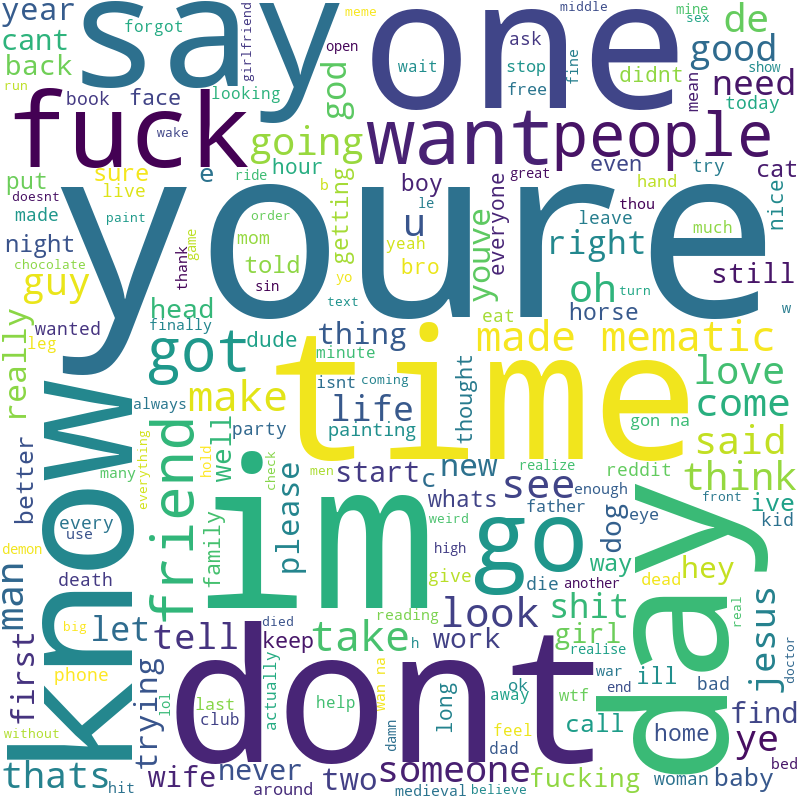
\includegraphics[scale=0.2]{acl18-latex/word_cloud_2022_ocr_text.png}
    \caption{Most frequent Words 2022}
    \label{fig:Word Cloud 2022}
\end{figure}

One possible explanation for this finding is perhaps the moderation of the subreddit. It may have become stricter, and pay more attention to the choice of words in memes. It may also be that the language of memes and the language of the internet has changed.
These explanations can only be verified by further analysis in similar meme subreddits or platforms and by statements from moderators.
\newline \par \textbf{Computer Vision}: In order to be able to make a comparison of the image brightness over the years, the years 2015, 2019 and 2022 (\autoref{fig: Colour 2015}, \ref{fig: Colour 2019}, \ref{fig: Colour 2022}) are shown below as examples.
\begin{figure}[H]
    \centering
    
\includegraphics[scale=0.6]{acl18-latex/Colour 2015.png}
    \caption{Color Barcode 2015}
    \label{fig: Colour 2015}
\end{figure}
\begin{figure}[H]
    \centering
    
\includegraphics[width=0.4\textwidth]{acl18-latex/Colour 2019.jpg}
    \caption{Color Barcode 2019}
    \label{fig: Colour 2019}
\end{figure}
\begin{figure}[H]
    \centering
    
\includegraphics[width=0.5\textwidth]{acl18-latex/2022_barcode.png}
    \caption{Color Barcode 2022}
    \label{fig: Colour 2022}
\end{figure}
If you look at the three barcode images, you can already guess that there is hardly any color difference between the years. To confirm this, we can look at the absolute brightness (\autoref{fig:Brightness}) of the meme images over the course of the years.
\begin{figure}[H]
    \centering
    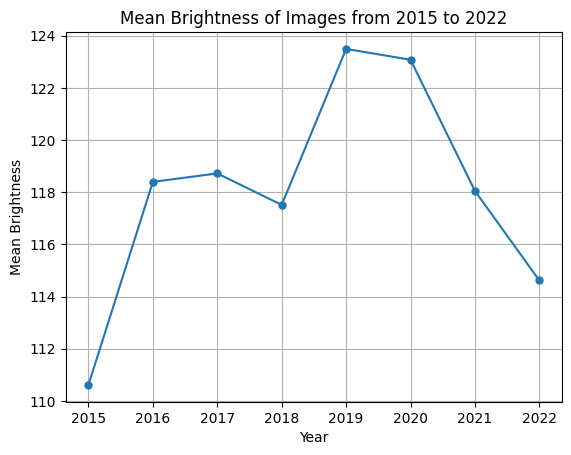
\includegraphics[scale=0.5]{acl18-latex/helligkeit in den jahren.png}
    \caption{Mean Brightness of Images from 2015-2022}
    \label{fig:Brightness}
\end{figure}
At first glance, there appears to be one or two changes in the average brightness of the images. The brightness increases in the years 2015 to 2019 and then decreases again until 2022. A closer look shows that the brightness changes from a value of 110 to about 124. The average brightness is calculated on the basis of the shades of grey. The shades of grey in the images are represented by a numerical scale from 0 to 255, with 0 being black and 255 being white. Considering the scale range, a change of 14 cannot be deemed significant. Therefore, it can be concluded that the images used in memes have maintained a consistent level of brightness over time.

 \section{Conclusion}
It was a challenge to collect the memes from Reddit and analyse the text, but with the help of OCR technology it was possible to study the memes. We focused on linguistic features such as NER, POS tagging and word frequency to gain insights into the language and content of the memes. The analysis of classical art memes showed that there were no significant differences in the use of linguistic and figurative features over time. The analysis of NER, POS tagging and word frequency showed no significant changes, suggesting that these memes will retain their relevance in the future.
Similarly, in the pictorial study, there were no significant changes in the colouring of the memes over time. This suggests that these visual characteristics are stable and unchanging in the use of classical art memes.
However, it was noticeable that the number of swear words decreased over time in the Reddit group studied. This could be due to improved moderation on Reddit.
Overall, the analysis of Classical Art memes shows that these memes are timeless and can have a lasting impact. Although there are no significant changes in the characteristics of the memes over time, these types of memes still provide an interesting area for the study of art and humour.
Our dataset provides a good basis for further analysis and research.. 
 
 \section{Limitation}
 The main limitation of this project, as described above, concerns the images. We were not able to identify the meme images based on image similarity and image corpora, nor were we able to identify the artists and names of the artworks. This problem was because of our data set. We would have to do a lot more image cleaning and possibly even hand searching. The collection of related work suggests that other researchers have also hand-searched the meme images for their analyses. Nevertheless, this project provides a good basis for further analysis and for finding the artwork.
Another limitation is the analysis of the texts. Our output gives a relatively neutral score for all memes. This is probably partly due to the fact that many words are not in the lexicon. There could be several reasons for this. On the one hand, it is certainly due to the fact that some of the words were misspelled or spelled differently (e.g. f*ck, sh*t). On the other hand, there are certain words that are trending (e.g. boomer) and have not yet been included in the lexicon. While NLTK-Vader is based on social media data, memes are still a separate category of social media language. Memes often consist of only half a sentence or, at most, two parts of a dialogue. Understanding the message of a meme requires text and images. Again, the text may be neutral and the image may give the message a negative or positive connotation.
However, our dataset provides a good basis for future analysis as it is very comprehensive with extensive meta data information.

 \section{Future Work}
 A prospect for future work could be further image analysis. The memes could be analysed using object and face recognition. For example, this could be used to find out whether the images are dominated by people, animals or objects. Similarly, face recognition can be used to analyse whether works of art by famous people such as the Mona Lisa, Marie Antoinette or Mozart are used. Another type of image analysis is image classification. This is a classification or categorisation of the individual artistic content, e. g. landscapes, portraits, everyday situations or abstract art. Further analysis can also include the examination of textures. It can be investigated whether materials can be represented in pictures and what attitudes people take.
 In addition to images, the subject of memes can also be analysed. This can include both images and language. In this way it can be examined whether politics is a constant theme or whether it only comes up when there is an election in a particular country. Similarly, seasonal topics (winter vs. summer) can be identified and the development of international topics (war, climate crisis, pandemic) can be studied in more detail. It might be interesting to see when these topics start to trend in the subreddits and when they start to decline.

% include your own bib file like this:
%\bibliographystyle{acl}
%\bibliography{acl2018}
\bibliography{acl2018}
\bibliographystyle{acl_natbib}

\end{document}

